\section{Validation and Sensitivity}\label{sec:validation}

A single worked example applied in this study illustrates that the computation recovers a known answer once. However, the results do not establish the accuracy of the uncertainty stated. To ensure accuracy of results, this section performs multiple replications of the example's data-generating process, varies its input, and investigates how often the reported 90\% band contains the true value of the avoided energy use. It also varies the life-cycle cost inputs. All analysis use the latest version 0.1.1 with its default model forms, selection rule, and acceptance criteria; Sec.~\ref{sec:changes} compares the results with version 0.1.0 on identical data. The scripts are described in Sec.~\ref{sec:avail}.

\subsection{Monte Carlo coverage of the Option C uncertainty}\label{sec:val_c}

\emph{Design.} Each replication draws a new 24-month baseline and 12-month reporting period from Eq.~(\ref{eq:dgp}) with the reference settings of Sec.~\ref{sec:example} ($F_{\rm true}=0.15$, $\sigma=12$ therms/day, temperature jitter 2.5\,F). It runs the entire Option C procedure and records the estimate $S_C$, the reported half-width $U_C$ at 80\%, 90\%, and 95\% confidence, the selected form, and the acceptance outcome. The truth in each replication is calculated as $F_{\rm true}$ times the noiseless baseline use at that replication's reporting temperatures. A replication is covered when $|S_C-S_{\rm true}|\le U_C$. For \McReps{} replications, the Monte Carlo standard error of a coverage near 90\% is about \McSeRef{} percentage points.

\emph{Results.} The estimator shows no detectable bias: the mean error is \McMeanErr{} therms against a mean true saving of \McMeanTrue{} therms, and the root-mean-square error is \McRmse{} therms. Empirical coverage is \McCovEighty\%, \McCovNinety\%, and \McCovNinetyFive\% at nominal 80\%, 90\%, and 95\%, each within about one Monte Carlo standard error of nominal (Fig.~\ref{fig:mc}). For monthly data generated without autocorrelation, the ASHRAE Guideline 14 approximation in Eq.~(\ref{eq:fsu}) is therefore well calibrated in this setting. This is consistent with the position that the approximation's known shortfalls arise mainly from autocorrelated residuals in daily and hourly models~\cite{touzani2019}, which this test does not include.

\begin{figure*}[t]
\centering
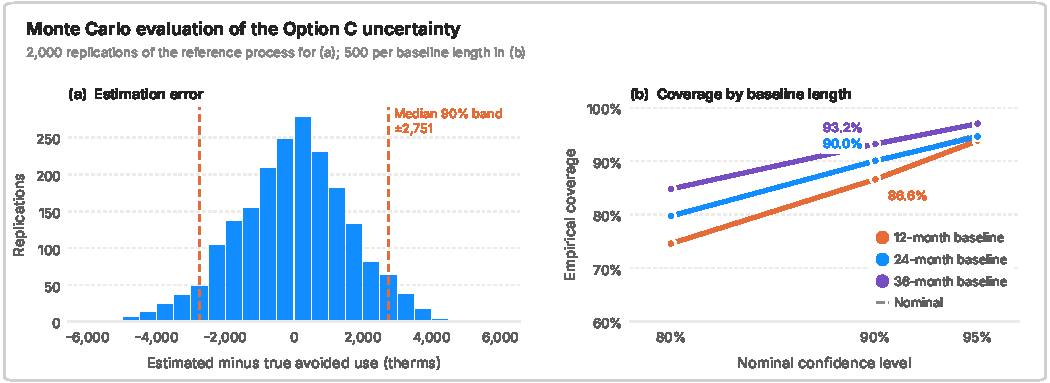
\includegraphics[width=\textwidth]{figs/fig_mc.pdf}
\caption{Monte Carlo evaluation of Option C. (a) Distribution of estimation error over \McReps{} replications of the reference process (bins of 500 therms); dashed lines mark the median reported 90\% half-width. (b) Empirical coverage of the reported uncertainty against the nominal confidence level for 12-, 24-, and 36-month baselines. The 24-month reference uses \McReps{} replications and the other two use \ScanReps{} each.}
\label{fig:mc}
\end{figure*}

\emph{Model selection.} The generating model is 3PH, and the selection rule chooses 3PH in \McFormThreePH\% of replications, 4P in \McFormFourP\%, and 5P in \McFormFiveP\%. The remaining over-parameterized choices occur when an extra slope passes the $|t|>2$ screen and also lowers the BIC, which happens by chance in a minority of noisy baselines. Coverage is \CovFormThreePH\% in the replications where 3PH is selected and \CovFormFourP\% where 4P is selected.

\emph{Acceptance outcomes.} Every replication passes the $R^2$, NMBE, slope-$t$, and CV(RMSE) criteria (median CV(RMSE) \McMedCv\%), and NMBE never exceeds $\McMaxNmbe$ percent, confirming that it is zero by construction under days-weighted least squares (Sec.~\ref{sec:optc}). This validation confirms that the NMBE criterion cannot fail for fits produced by the toolkit. The binding criterion is FSU: \McPass\% of replications pass all criteria, and every failure is an FSU above 50\%. The worked example's FSU of \FSU\% is therefore not unusual; the median over replications is \McMedFsu\%.

\subsection{Changes in version 0.1.1}\label{sec:changes}

The same tests were initially conducted on version 0.1.0 where two behaviors were identified and corrected in Version 0.1.1. Table~\ref{tab:changes} compares both versions from identical data.

\emph{Model selection.} Version 0.1.0 selected the significant-slope model using the lowest CV(RMSE). For the reference process, it chose a 4P or 5P model in \BeforeNonThree\% of replications. Since each slope's $t$-statistic is computed conditional on a change point that was chosen to minimize error, the $|t|>2$ screen admits a spurious slope more often than its nominal level implies, and CV(RMSE) penalizes an added parameter only through $n-p$. The over-fitted models reported a lower CV(RMSE) and understated their own uncertainty. With selections by BIC, Eq.~(\ref{eq:bic}), penalizes each added parameter by $\ln n$. It reduced the over-parameterized choices to \AfterNonThree\%, raised coverage at 90\% from \BeforeCovNinety\% to \McCovNinety\%, and lowered the RMSE from \BeforeRmse{} to \McRmse{} therms. To ascertain that the stricter rule does not underfit, the test was repeated on processes whose true model is 4P or 5P. For a true 4P model the two rules perform alike. For a true 5P model, BIC identifies the 5P form less often (\UfFivePAfter\% against \UfFivePBefore\%), but the RMSE of the savings estimate changed by only \UfFivePRmseChange\% and coverage is \UfFivePCovAfter\% against \UfFivePCovBefore\%. For this process, the effect on the savings estimate is considerably small.

\emph{Uncertainty for non-positive savings.} Version 0.1.0 computed the absolute uncertainty as FSU times savings and therefore reported none when estimated savings were zero or negative, which occurred in \BeforeUndefFive\% of replications at 5\% true savings. Version 0.1.1 computes $U_C$ directly from Eq.~(\ref{eq:uc}), which does not involve savings, so a report can state that savings were not distinguishable from zero. Coverage at 5\% true savings rises from \BeforeCovFive\% to \CovFrFive\%, and at $\sigma=36$ from \BeforeCovNoise\% to \CovNoiseThirtySix\%.

Neither change affects the worked example: its candidate models rank the same under both rules highlighted in (Table~\ref{tab:cand}), and its savings are positive.

\begin{table}[t]
\caption{Option C results based on identical synthetic data under versions 0.1.0 and 0.1.1. The reference process has a true 3PH model ($F_{\rm true}=15\%$, $\sigma=12$ therms/day, 24-month baseline, \McReps{} replications); the weak and noisy rows use \ScanReps{} replications each.}
\label{tab:changes}
\centering\small
\begin{tabular}{@{}lrr@{}}
\toprule
 & v0.1.0 & v0.1.1 \\
\midrule
\multicolumn{3}{@{}l}{\emph{Reference process, true model 3PH}} \\
\BeforeAfterRows
\bottomrule
\end{tabular}
\end{table}

\subsection{Dependence on savings size, noise, and baseline length}

Table~\ref{tab:scan} varies one setting at a time with \ScanReps{} replications each (Monte Carlo standard error about \McSeScan{} points at 90\%). Within each block the same random draws are reused across settings, so differences between rows reflect the setting rather than sampling.

\begin{table*}[t]
\caption{Option C performance as one setting is varied from the reference ($F_{\rm true}=15\%$, $\sigma=12$ therms/day, 24-month baseline). Errors are in therms. Coverage is the share of replications in which the reported band contains the truth. The last column is the share of replications where the estimated savings are zero or negative; the absolute uncertainty is still reported for them, but FSU is not, and they fail the FSU criterion.}
\label{tab:scan}
\centering\small
\begin{tabular}{@{}lrrrrrrrr@{}}
\toprule
Setting & Mean error & RMSE & Median FSU$_{90}$ (\%) & Cov.\ 80\% & Cov.\ 90\% & Cov.\ 95\% & Pass all (\%) & $S_C\le0$ (\%) \\
\midrule
\ScanRows
\bottomrule
\end{tabular}
\end{table*}

\emph{Savings fraction.} Error and absolute uncertainty do not change with $F_{\rm true}$, as Eq.~(\ref{eq:fsu}) implies (Sec.~\ref{sec:fsu}): the RMSE is the same in every row of the block. The noticeable change in every block is the FSU, from a median of \MedFsuFive\% at 5\% savings to \MedFsuThirty\% at 30\%, together with the acceptance rate, from \PassFrTen\% at 10\% savings to \PassFrTwenty\% at 20\%. In practical applications, the FSU criterion in Table~\ref{tab:accept} determines whether a project of this size and noise level can be verified at all from monthly bills. At 5\% savings, the estimate is zero or negative in \NonposFive\% of replications; the band is still reported, and coverage is \CovFrFive\%.

\emph{Noise.} By halving the noise to $\sigma=6$, the RMSE is instantaneously halved (\RmseNoiseSix{} therms) and every replication passes. At $\sigma=36$ the RMSE is \RmseNoiseThirtySix{} therms and only \CvOkNoiseThirtySix\% of replications meet the CV(RMSE) criterion, but the coverage stays at or above nominal in all noise settings: noticeably, the band widens with the noise as it should.

\emph{Baseline length.} A 12-month baseline raises the RMSE to \RmseYrOne{} therms and lowers coverage to \CovYrOne\% at nominal 90\% and \CovYrOneEighty\% at nominal 80\%, an indicator that the approximation is somewhat optimistic for the shortest baseline acceptable by FEMP v5.0. A 36-month baseline lowers the RMSE to \RmseYrThree{} therms, and coverage of \CovYrThree\% is slightly conservative. These results support the FEMP v5.0 guidance to use whole-year baselines, suggestive that one year baseline should be treated as a minimum rather than a target.

\subsection{Option A coverage}\label{sec:val_a}

The worked example's exact Option A match is built into the example (Sec.~\ref{sec:example}). To test Eq.~(\ref{eq:opta_unc}), we drew \OaReps{} replications of five readings before and after the retrofit from normal distributions with means of 14.6 and 6.2 kW and a standard deviation of \OaSd\,kW, with the operating hours fixed at their stipulated value. Coverage is \OaCovEighty\%, \OaCovNinety\%, and \OaCovNinetyFive\% at nominal 80\%, 90\%, and 95\%, and the median relative uncertainty at 90\% is \OaMedRel\%. This result confirms the arithmetic of the interval for independent, normally distributed readings. It records no information about the uncertainty in stipulated hours, which the toolkit does not quantify by design.

\subsection{Sensitivity of the life-cycle cost results}\label{sec:val_lcc}

\emph{Propagation of measured-savings uncertainty.} Each verified therm of gas savings calculated in this replication is worth \$\NsPerTherm{} of net present value over the study period. When both verified quantities are moved to the edges of their 90\% bands (gas $\pm$\AbsUnc{} therms, lighting $\pm$\OptAUnc{} kWh), the net savings increases from \$\NsLow{} to \$\NsHigh{} and the SIR from \SirLow{} to \SirHigh. Across the band, the cost-effectiveness verdict remains unchanged across the band, but its size is uncertain by roughly a third in either direction, which a report derived from a single projected savings would not have shown.

\emph{Discount rate, energy price, and study period.} Fig.~\ref{fig:lcc} varies one input at a time for each replication. Net savings fall with the real discount rate and reach zero at \BeRate\%, where the adjusted internal rate of return (AIRR) equals the discount rate as indicated in Eq.~(\ref{eq:airr}). Net savings becomes positive in a study period of \BeYears{} years, then increases linearly with the gas price, and remains consistently positive (\$\NsZeroGas) even at a gas price of zero.

In this synthetic worked example, the avoided base-case boiler replacement and the lighting and maintenance savings exceed the added investment on their own. This further establishes that the verified gas savings worth about \$\GasSavPV{} in the present value, determine the size of the net savings rather than its positive or negative sign.

\begin{figure*}[t]
\centering
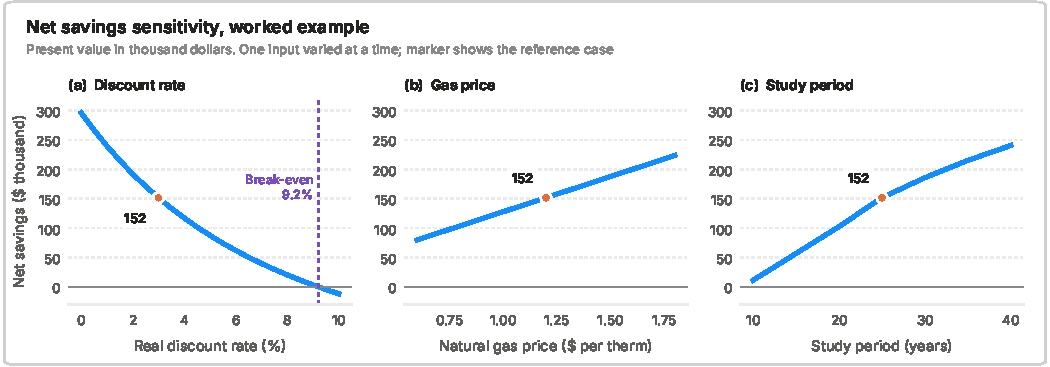
\includegraphics[width=\textwidth]{figs/fig_lcc.pdf}
\caption{Net savings of the worked example as one life-cycle cost input is varied: (a) real discount rate, (b) natural gas price, (c) study period. The orange marker is the reference case (3.0\%, \$1.20 per therm, 25 years; net savings \$\NetSavings); the dotted line in (a) marks the break-even rate.}
\label{fig:lcc}
\end{figure*}

\section{Limitations and Scope}\label{sec:limits}

There are four core measurement and verification options defined by IPMVP. Of these options, the toolkit implements two of the four IPMVP options: Options A (key parameter measurement) and C (whole facility). Option B (all parameters measured) and Option D (calibrated simulation) are not implemented in this toolkit. Option C uses temperature as the only independent variable, other variables such as occupancy, school calendars, and production are not modeled. Non-routine adjustments must be estimated outside the toolkit and documented in the M\&V plan. Avoided energy use is computed, but normalized savings is not accounted for. The uncertainty method applied is the ASHRAE Guideline 14 approximation for monthly data rather than the EVO 10100-1:2018 procedure cited in FEMP v5.0; it does not correct for autocorrelation and should not be applied to daily or hourly data without that correction~\cite{touzani2019,walter2014}. The 1.26 constant used in the toolkit has not been verified against a licensed copy of the 2023 guideline. The Monte Carlo results in Sec.~\ref{sec:validation} is based on a data-generating process that matches the 3PH model family, has independent Gaussian errors, and has no non-routine events, so they present calibration under favorable conditions. They do not represent as evidence of performance on real municipal billing data, which has not yet been tested in this toolkit. Life-cycle cost is calculated in constant dollars; taxes, financing, and incentives as cash flows are not modeled. Finally, the report module organizes the content as specified in 2 CFR 200.329 and checks its completeness. It is not a compliance determination procedure and does not replace the form prescribed by the awarding agency, and it does not model due-date extensions.

\section{Concluding Remarks}\label{sec:conclusion}

MUNI-LCC is a compact open access toolkit designed to implement the performance reporting process for energy efficiency upgrades, from metered data to a federal performance report based on IPMVP Options A and C as defined in FEMP v5.0, life-cycle cost consistent with ASTM E917, and content elements of 2 CFR 200.329. The integral essence for the development of the toolkit is to ensure that verified quantities, not projections, are computed into the life-cycle cost study so that Net Savings (NS), Savings-to-Investment Ratio (SIR), Adjusted Internal Rate of Return (AIRR), and unit cost are accurately reported on a measured basis with every acceptance value referencing its source.

Based on observation from the synthetic example with a known answer, it is confirmed that the toolkit recovers the injected gas savings within its stated uncertainty. Across \McReps{} replications of the same process, the Option C uncertainty attains coverage of \McCovNinety\% at a nominal 90\% with no detectable bias, and Option A coverage is likewise close to nominal. Findings from the tests in version 0.1.0 justified the need for two changes which was implemented in version 0.1.1. The two changes include: model selection by information criterion, which cuts spurious change-point models from \BeforeNonThree\% to \AfterNonThree\% of replications; and an absolute uncertainty reported for any sign of savings. Neither of these changes altered the worked example. The tests further validate that the FSU criterion, not the model fit, decides whether a modest saving can be verified from the monthly bills.

Future scope of work will include the integration of Option B (all parameter measurement), the EVO 10100-1:2018 uncertainty procedure alongside the current approximation, normalized savings, and additional independent variables, validated against real municipal billing data compared against an established open M\&V implementation on the same data.

\section*{Code and Data Availability}\label{sec:avail}

The MUNI-LCC source code, documentation, synthetic example data, and tests are packaged in a repository publicly accessible at \url{https://github.com/Olumide-Akindipe/muni-lcc} under the MIT license (documentation CC BY 4.0). The manuscript source and the scripts supporting every table and figure in this paper (\code{validation.py}, \code{underfit\_check.py}, \code{lcc\_scans.py}, \code{figures.py}, and \code{make\_numbers.py}, which writes every number in the text from the output files) are in the \code{preprint/} folder of the repository, together with their outputs. Version 0.1.0 is archived on Zenodo~\cite{munilcc}, and every version, including 0.1.1, is available under the concept DOI 10.5281/zenodo.23362541. Real utility data are not used.

\section*{Competing Interests}

The author declares no competing interests.

\section*{Acknowledgment}

No financial support was received for this work.

\bibliographystyle{unsrtnat}
\bibliography{refs}
